\documentclass[aspectratio=169]{beamer}

% 引入中文支持和数学包
\usepackage[UTF8]{ctex}
\usepackage{amsmath}
\usepackage{amssymb}
\usepackage{booktabs}
\usepackage{bm}
\usepackage{graphicx} % 用于插入图片
\usepackage{hyperref} % 用于 \url 可点击链接
\graphicspath{{figs/}} % 图片目录；请务必在 file_3_16 目录下编译

% 设置南大紫主题色 (提取自图片参考)
\definecolor{NJUPurple}{RGB}{84, 18, 84}
\usetheme{Madrid}
\usecolortheme[named=NJUPurple]{structure}

% 隐藏导航符号
\setbeamertemplate{navigation symbols}{}

% 标题页信息
\title{题目1：机器学习正则化中的范数应用}
\subtitle{矩阵计算与优化汇报}
\institute{第19组}
\date{2025年3月18日}

\begin{document}

% --- 封面 ---
\begin{frame}
    \titlepage
\end{frame}

% --- 题目总览 (提取自图片) ---
\begin{frame}{题目背景总览}
    \textbf{对应知识点：}向量范数、矩阵范数、范数等价性
    \vspace{0.3cm}
    
    \textbf{场景背景（如金融风控、医疗特征建模）：}线性回归 L1/L2 正则化，特征矩阵 $X \in \mathbb{R}^{m \times n}$，标签 $y$，参数 $\beta$。
    
    $$J_1(\beta) = \frac{1}{2m} \|X\beta - y\|_2^2 + \lambda \|\beta\|_1$$
    $$J_2(\beta) = \frac{1}{2m} \|X\beta - y\|_2^2 + \lambda \|\beta\|_2^2$$
    
    \vspace{0.3cm}
    \textbf{解题角度：}
    \begin{enumerate}
        \item 解释范数意义，说明稀疏性差异
        \item 证明有限维空间范数等价性
        \item 数值实验对比两种正则化
        \item 分析 F 范数的数值稳定性优势
    \end{enumerate}
\end{frame}


% ==========================================
% 角度1：解释范数意义，说明稀疏性差异
% ==========================================
\section{解释范数意义，说明稀疏性差异}

% --- 衔接页 1 ---
\begin{frame}{内容大纲 \& 环节过渡}
    \tableofcontents[currentsection]
    \vspace{0.5cm}
    \begin{block}{本节导读：}
        “本部分旨在从直观层面阐述机器学习中正则化机制的核心作用，并结合具体案例，剖析 L1 与 L2 正则化在约束模型参数时产生不同分布特性（特别是稀疏性差异）的物理意义与内在逻辑。”
    \end{block}
\end{frame}

\begin{frame}{背景补全：机器学习是在干什么？}
    假设我们手头有南京市过去 10 年的房价数据，包含：\textbf{面积、地段、楼层、甚至房东的星座}。我们的目标是：给出一个新房子的信息，让模型预测它值多少钱。
    \begin{enumerate}
        \item \textbf{建立模型}：\\
        我们假设价格 $y$ 和这些因素 $x$ 之间有一个简单的线性关系：
        $$\text{价格} = \beta_1 \cdot \text{面积} + \beta_2 \cdot \text{地段} + \beta_3 \cdot \text{楼层} + \beta_4 \cdot \text{星座} \dots$$
        这里的 $\beta$（参数）就是我们要让电脑“学”出来的秘密配方。
        
        \item \textbf{什么是“学习”？}\\
        所谓学习，就是不断调整 $\beta$ 的数值，让预测出来的价格和实际成交价格$y$的\textbf{误差（Loss）}最小。
        \begin{itemize}
            \item 这里我们把预测误差定义为 $J(\beta)$ 前半部分的 $\frac{1}{2m}\|X\beta - y\|_2^2$ 
            \item 即 $\text{Loss} = \frac{1}{2m}\|X\beta - y\|_2^2$
        \end{itemize}
    \end{enumerate}
\end{frame}

\begin{frame}{过拟合现象}
    \begin{block}{核心冲突：“如果模型太想拿高分了，会发生什么？”}
        \begin{itemize}
            \item \textbf{例子}：模型发现，在过去的数据里，凡是房东是“处女座”的房子都贵了 5 万块。于是它把 $\beta_4$（星座权重）设得很大。
            \item \textbf{后果}：在旧数据上，预测确实很准；但拿去预测明天的新房子时，发现根本不准。因为“星座”和“房价”根本没关系，那只是旧数据里的\textbf{随机噪声}。
        \end{itemize}
    \end{block}
    \vspace{0.5cm}
    \textbf{结论：}这种现象叫“过拟合”。模型为了迎合旧数据，学习了一堆乱七八糟、没有规律的“废话”。
\end{frame}

\begin{frame}{正则化与新的损失函数}
    为了防止过拟合，我们引入正则化。
    
    \vspace{0.5cm}
    \textbf{新的损失函数}：
    \begin{block}{L1 正则化损失函数}
        $$J_1(\beta) = \frac{1}{2m} \|X\beta - y\|_2^2 + \lambda \|\beta\|_1$$
    \end{block}
    \begin{block}{L2 正则化损失函数}
        $$J_2(\beta) = \frac{1}{2m} \|X\beta - y\|_2^2 + \lambda \|\beta\|_2^2$$
    \end{block}
\end{frame}

\begin{frame}{从参数更新角度解释稀疏性}
    在机器学习中，模型通过不断调整参数 $\beta$ 来减小误差。这个调整的过程叫做\textbf{梯度下降}。
    
    \begin{block}{比喻：浓雾中下山}
        想象你被困在一个充满浓雾的山坡上，看不见远处的山谷（最低点/最优解），你只能看清脚下的一小块地。
        \begin{itemize}
            \item \textbf{梯度}：就是你脚下土地的\textbf{坡度}（陡峭程度）。
            \item \textbf{下降}：你踩了踩地，发现往左前方走坡度最陡，于是你朝那个方向迈出一小步。
            \item \textbf{训练过程}：你每走一步，就重新感知一下坡度，再迈一步。经过成百上千步后，你最终会到达山底。
        \end{itemize}
    \end{block}

    \textbf{参数更新公式}：\\
    模型每一步更新参数的逻辑是：
    \begin{quote}
        \textbf{新权重 = 旧权重 - 调整力度 (学习率) $\times$ 梯度}
    \end{quote}
\end{frame}

\begin{frame}{1. L2 正则化 ($\beta^2$)：像是“弹簧拉力”}
    \begin{itemize}
        \item \textbf{拉力大小}：L2 的梯度（导数）是 $2\beta$。这意味着\textbf{拉力的大小和 $\beta$ 的数值成正比}。
        \item \textbf{力学表现}：
        \begin{itemize}
            \item 当 $\beta$ 很大时，弹簧被拉得很长，产生巨大的拉力，迅速把它往回拽。
            \item \textbf{关键点}：当 $\beta$ 变得非常小（接近 0）时，弹簧几乎不再形变，\textbf{拉力也随之消失了}。
        \end{itemize}
        \item \textbf{结果}：对于“房东星座”这种无关特征，L2 觉得只要把它压得足够小（比如 0.000001），它对房价的影响就忽略不计了，没必要非得把它拽到 0。所以，\textbf{L2 产出的参数大多很小，但一般不为0}。
    \end{itemize}
\end{frame}

\begin{frame}{2. L1 正则化 ($|\beta|$)：像是“恒定推力”}
    \begin{itemize}
        \item \textbf{拉力大小}：L1 的梯度（导数）是固定常数 $1$ 或 $-1$。这意味着\textbf{无论 $\beta$ 多大多小，拉力永远是恒定的}。
        \item \textbf{力学表现}：
        \begin{itemize}
            \item 即使 $\beta$ 已经缩小到了 0.000001，L1 施加的力依然是稳稳的 “1”。
        \end{itemize}
        \item \textbf{结果}：这个恒定的能力直接把无关紧要的参数（如“房东星座”）减小到0并锁死。所以，\textbf{L1 产出的参数中，会有很多正好等于 0}，即呈现出稀疏性。
    \end{itemize}
\end{frame}


% ==========================================
% 角度2：证明有限维空间范数等价性
% ==========================================
\section{证明有限维空间范数等价性}

% --- 衔接页 2 ---
\begin{frame}{内容大纲 \& 环节过渡}
    \tableofcontents[currentsection]
    \vspace{0.5cm}
    \begin{block}{章节过渡：}
        “尽管 L1 与 L2 正则化在优化结果上呈现出显著的宏观差异，但从底层数学结构的角度来看，二者在有限维空间中具有深层的内在联系。本部分将基于严格的数学定义，推导并证明 $\mathbb{R}^n$ 空间中 1-范数与 2-范数的等价关系。”
    \end{block}
\end{frame}

\begin{frame}{一、范数等价性的定义}
    \begin{block}{\textbf{定义：范数等价（Norm Equivalence）}}
        设 $V$ 是有限维向量空间。\\
        若两个范数 $\|\cdot\|_a$ 与 $\|\cdot\|_b$ 满足
        $$ c_1\|x\|_a \le \|x\|_b \le c_2\|x\|_a $$
        其中 $c_1>0, c_2>0$，且对所有 $x\in V$ 成立，\\
        则称这两个范数 \textbf{等价}。
    \end{block}
    
    \textbf{重要结论：}在有限维空间中，任意两个范数都是等价的。
    
    \vspace{0.3cm}
    本题需要证明：在 $\mathbb{R}^n$ 中，
    $$ \|x\|_1 \sim \|x\|_2 $$
    即 $L_1$ 范数与 $L_2$ 范数等价。
\end{frame}

\begin{frame}{二、1范数与2范数定义}
    设
    $$ x=(\beta_1,\beta_2,\dots,\beta_n) $$
    
    \begin{block}{1范数（L1 norm）}
        $$ \|x\|_1=\sum_{i=1}^{n}|\beta_i| $$
    \end{block}

    \begin{block}{2范数（L2 norm）}
        $$ \|x\|_2=\sqrt{\sum_{i=1}^{n}\beta_i^2} $$
    \end{block}
\end{frame}

\begin{frame}{三、范数等价性证明 - (1) 证明 $\|x\|_2 \le \|x\|_1$}
    需要证明两个不等式。首先证明：$$ \|x\|_2 \le \|x\|_1 $$
    
    因为：
    $$ \left(\sum_{i=1}^{n}|\beta_i|\right)^2 = \sum_{i=1}^{n}\beta_i^2 +2\sum_{i<j}|\beta_i||\beta_j| $$
    
    显然：
    $$ \left(\sum_{i=1}^{n}|\beta_i|\right)^2 \ge \sum_{i=1}^{n}\beta_i^2 $$
    
    两边开平方得到：
    $$ \sqrt{\sum_{i=1}^{n}\beta_i^2} \le \sum_{i=1}^{n}|\beta_i| $$
    
    即：
    $$ \|x\|_2 \le \|x\|_1 $$
\end{frame}

\begin{frame}{三、范数等价性证明 - (2) 证明 $\|x\|_1 \le \sqrt{n}\|x\|_2$}
    证明：$$ \|x\|_1 \le \sqrt{n}\|x\|_2 $$
    
    利用 \textbf{柯西–施瓦茨不等式（Cauchy–Schwarz）}：
    $$ \left(\sum_{i=1}^{n}|\beta_i|\right)^2 \le \left(\sum_{i=1}^{n}1^2\right) \left(\sum_{i=1}^{n}\beta_i^2\right) $$
    
    因为 $\sum_{i=1}^{n}1^2=n$，所以：
    $$ \left(\sum_{i=1}^{n}|\beta_i|\right)^2 \le n\sum_{i=1}^{n}\beta_i^2 $$
    
    开平方得到：
    $$ \sum_{i=1}^{n}|\beta_i| \le \sqrt{n}\sqrt{\sum_{i=1}^{n}\beta_i^2} $$
    
    即：
    $$ \|x\|_1 \le \sqrt{n}\|x\|_2 $$
\end{frame}

\begin{frame}{四、最终结果 \& 五、与机器学习正则化的联系}
    综合两个不等式：
    $$ \|x\|_2 \le \|x\|_1 \le \sqrt{n}\|x\|_2 $$
    因此存在常数 $c_1=1,\quad c_2=\sqrt{n}$，使得 $c_1\|x\|_2 \le \|x\|_1 \le c_2\|x\|_2$。
    
    \textbf{结论：}在有限维空间 $\mathbb{R}^n$ 中，$\|\cdot\|_1 \sim \|\cdot\|_2$，即 \textbf{1范数与2范数等价}。
    
    \vspace{0.4cm}
    L1 范数与 L2 范数都可以作为机器学习中的正则化项，用于限制模型参数大小。
    
    \begin{table}[]
        \centering
        \begin{tabular}{|l|l|}
        \hline
        \textbf{方法} & \textbf{作用} \\ \hline
        L1 正则化 & 产生稀疏解（许多参数变为 0），常用于特征选择 \\ \hline
        L2 正则化 & 使参数整体变小，但通常不会变为 0 \\ \hline
        \end{tabular}
    \end{table}
    
    因此：\textbf{两种正则化理论目标一致，但优化结果不同。}
\end{frame}

% --- 一般范数等价性：定理与证明思路 ---
\begin{frame}{推广：有限维空间上任意范数等价定理}
    \begin{block}{\textbf{定理（范数等价）}}
        设 $V$ 是 $\mathbb{R}$ 或 $\mathbb{C}$ 上的\textbf{有限维}向量空间。对 $V$ 上任意两个范数 $\|\cdot\|_a$ 与 $\|\cdot\|_b$，存在正常数 $C_1,\,C_2$，使得对所有 $v \in V$：
        \[
        C_1 \|v\|_b \le \|v\|_a \le C_2 \|v\|_b.
        \]
        此时称 $\|\cdot\|_a$ 与 $\|\cdot\|_b$ \textbf{等价}。
    \end{block}
    \vspace{0.3cm}
    \textbf{证明思路：}
    \begin{enumerate}
        \item 取“参考范数”（通常取 $\|\cdot\|_2$）。
        \item 证明任意范数 $\|\cdot\|$ 都与 $\|\cdot\|_2$ 等价。
        \item 由等价关系的传递性，任意两个范数彼此等价。
    \end{enumerate}
\end{frame}

\begin{frame}{一般等价性证明 (1)：存在上界 $C_2$}
    设 $\dim V = n$，取基 $\{e_1,\dots,e_n\}$，则 $v = \sum_{i=1}^n x_i e_i$。定义参考范数 $\|v\|_2 := \big(\sum_i |x_i|^2\big)^{1/2}$。

    对任意范数 $\|\cdot\|$，由三角不等式与柯西—施瓦茨不等式：
    \[
    \|v\| = \Big\|\sum_{i=1}^n x_i e_i\Big\| \le \sum_{i=1}^n |x_i| \|e_i\|
    \le \Big(\sum_{i=1}^n |x_i|^2\Big)^{\!1/2} \Big(\sum_{i=1}^n \|e_i\|^2\Big)^{\!1/2} = C_2 \|v\|_2,
    \]
    其中 $C_2 = \big(\sum_{i=1}^n \|e_i\|^2\big)^{1/2}$ 为与 $v$ 无关的正常数。故 $\|v\| \le C_2 \|v\|_2$ 对所有 $v$ 成立。
\end{frame}

\begin{frame}{一般等价性证明 (2)：存在下界 $C_1$（关键步骤）}
    考虑单位球面 $S = \{ v \in V : \|v\|_2 = 1 \}$。$f(v)=\|v\|$ 在 $S$ 上连续，$S$ 在有限维 $\|\cdot\|_2$ 下为\textbf{有界闭集}（紧集），故 $f$ 在 $S$ 上取得最小值：
    \[
    m = \min_{v \in S} \|v\|.
    \]
    $S$ 中向量非零，由范数正定性知 $m > 0$。

    对任意非零 $v$，令 $u = v/\|v\|_2 \in S$，则 $\|v\| = \|v\|_2 \cdot \|u\| \ge \|v\|_2 \cdot m$。取 $C_1 = m$，即得 $C_1 \|v\|_2 \le \|v\|$ 对所有 $v$ 成立。

    \vspace{0.2cm}
    \textbf{直观：} 单位球面上连续函数必有正的最小值，故新范数不会无限趋近于 0。
\end{frame}

\begin{frame}{一般范数等价：总结与意义}
    综上，任意范数 $\|\cdot\|$ 都与 $\|\cdot\|_2$ 等价：$C_1 \|v\|_2 \le \|v\| \le C_2 \|v\|_2$。由传递性，$V$ 上所有范数相互等价。

    \vspace{0.3cm}
    \textbf{意义：}
    \begin{itemize}
        \item 有限维中收敛性、连续性、开/闭集、完备性等与具体范数选取无关。
        \item 可选用最方便的范数（如欧几里得范数）进行研究。
        \item 该结论对\textbf{无限维}空间不成立——那里存在不等价的范数。
    \end{itemize}
\end{frame}


% ==========================================
% 角度3：数值实验对比两种正则化
% ==========================================
\section{数值实验对比两种正则化}

% --- 衔接页 3 ---
\begin{frame}{内容大纲 \& 环节过渡}
    \tableofcontents[currentsection]
    \vspace{0.5cm}
    \begin{block}{章节过渡：}
        “前期的理论推演确立了不同范数在有限维空间中的有界性关系与作用机理。为进一步验证理论推导在实际计算环境中的表现，本部分将引入数值实验，在具体数据集下量化对比两种正则化的收敛过程与参数稀疏度指标。”
    \end{block}
\end{frame}

\begin{frame}{主实验：高维稀疏合成数据设定}
    \textbf{实验目标：} 验证高维稀疏特征场景下 L1 与 L2 范数惩罚的效果差异。
    
    \vspace{0.3cm}
    \textbf{实验设定：}
    \begin{itemize}
        \item \textbf{数据规模}：150 个样本，200 个特征（属于典型的 $n < m$ 高维场景）。
        \item \textbf{真实分布}：在 200 个特征中，仅 \textbf{10 个特征具有真实的非零系数}（强稀疏假设）。
        \item \textbf{处理流程}：数据标准化后，按 7:3 划分为训练集与测试集。通过在测试集上的均方误差（MSE）来选定最佳正则化强度 $\lambda$。
    \end{itemize}
    
    \vspace{0.3cm}
    \textbf{核心结论（概览）：}
    Lasso 在预测误差上表现更优，并成功精准锁定了极少数的非零特征；而 Ridge 整体缩小了所有参数，但并未实现特征剔除。这与我们在“角度一”中的理论推导完美契合。
\end{frame}

\begin{frame}{测试集 MSE 随正则化强度 $\lambda$ 的变化}
    \centering
    
\includegraphics[height=0.65\textheight]{figs/fig1_mse_vs_lambda.png}\\
    \footnotesize Lasso（蓝）在某个最佳 $\lambda$ 处达到远低于 Ridge（橙）的测试 MSE。
\end{frame}

\begin{frame}{正则化路径对比：稀疏性 vs 整体收缩}
    \begin{columns}[T]
        \begin{column}{0.48\textwidth}
            \centering
            
\includegraphics[width=\linewidth]{figs/fig2_lasso_coef_path.png}\\
            \footnotesize \textbf{Lasso：}随 $\lambda$ 增大，无关系数被压成 0。
        \end{column}
        \begin{column}{0.48\textwidth}
            \centering
            
\includegraphics[width=\linewidth]{figs/fig3_ridge_coef_path.png}\\
            \footnotesize \textbf{Ridge：}系数整体变小，但不为 0。
        \end{column}
    \end{columns}
\end{frame}

\begin{frame}{最佳 $\lambda$ 下的最终系数分布对比}
    \centering
    
\includegraphics[height=0.6\textheight]{figs/fig4_coef_compare.png}\\
    \footnotesize Lasso 贴合真实稀疏特征，Ridge 系数密集非零。
\end{frame}

\begin{frame}{模型预测性能深度评估}
    \begin{columns}[T]
        \begin{column}{0.48\textwidth}
            \centering
            
\includegraphics[width=\linewidth]{figs/fig5_residual_boxplot.png}\\
            \footnotesize 残差箱线图：Lasso 更集中于 0 附近。
        \end{column}
        \begin{column}{0.48\textwidth}
            \centering
            
\includegraphics[width=\linewidth]{figs/fig6_pred_vs_true.png}\\
            \footnotesize 预测 vs 真实：Lasso 更贴对角线。
        \end{column}
    \end{columns}
\end{frame}

\begin{frame}{辅助实验：真实数据分布中的教训（BlogFeedback）}
    \textbf{实验背景：} BlogFeedback 真实数据（280 维，预测评论数），$y$ 分布极偏、长尾。
    \begin{columns}[T]
        \begin{column}{0.48\textwidth}
            \centering
            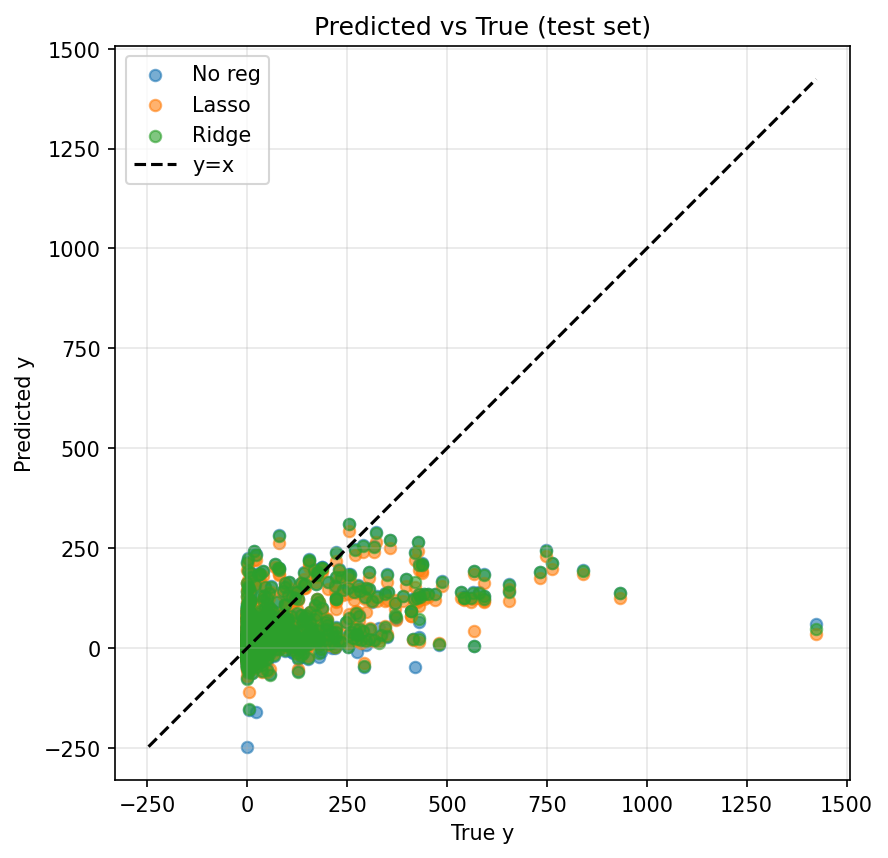
\includegraphics[width=\linewidth]{figs/exp2_noLog_fig6_pred_vs_true.png}\\
            \footnotesize \textbf{未取对数：}预测 vs 真实散点严重偏离 $y=x$，高真实值被严重低估，存在极大误差。
        \end{column}
        \begin{column}{0.48\textwidth}
            \centering
            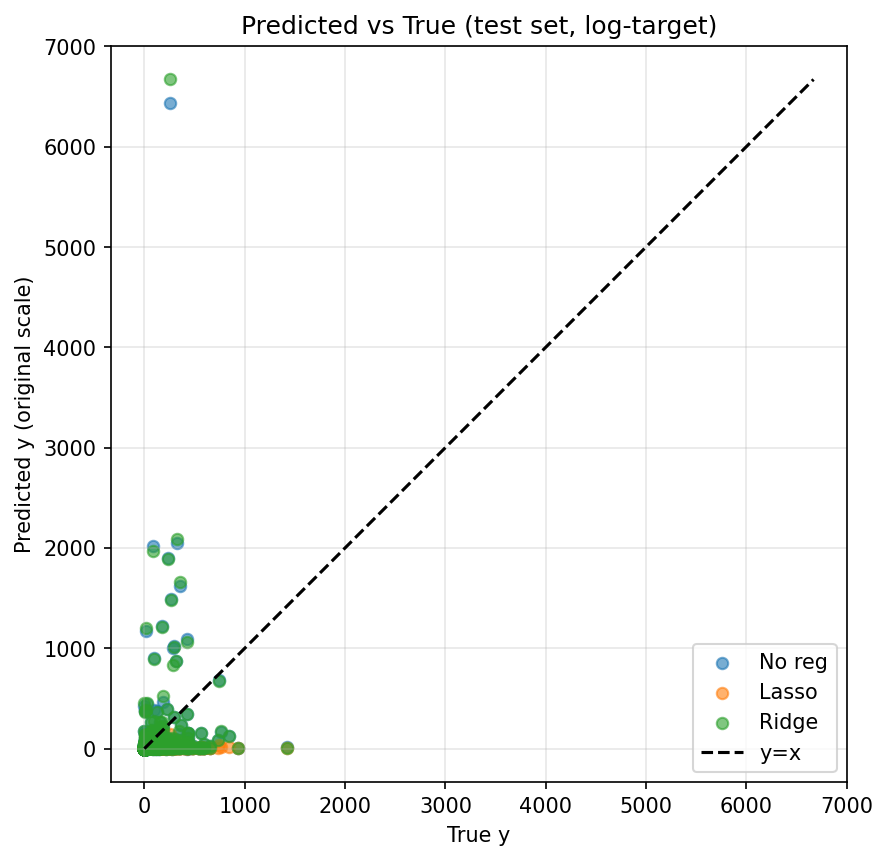
\includegraphics[width=\linewidth]{figs/exp2_log_fig6_pred_vs_true.png}\\
            \footnotesize \textbf{取对数后：}对目标做 $\log(1+y)$ 再建模仍存在极大误差（过预测/欠预测明显），说明单靠正则化不足，需数据与评估手段配合。
        \end{column}
    \end{columns}
    \vspace{0.2cm}
    \footnotesize \textbf{教训：} 真实场景需数据预处理与鲁棒评估指标，单纯范数正则化不够。
\end{frame}


% ==========================================
% 角度4：分析 F 范数的数值稳定性优势
% ==========================================
\section{分析 F 范数的数值稳定性优势}

% --- 衔接页 4 ---
\begin{frame}{内容大纲 \& 环节过渡}
    \tableofcontents[currentsection]
    \vspace{0.5cm}
    \begin{block}{章节过渡：}
        “前述讨论主要针对参数以向量形式存在的单输出回归场景。随着模型结构的复杂化（如多输出回归与深度神经网络），参数通常升维为矩阵结构。本部分将约束条件拓展至矩阵范数，重点剖析 Frobenius 范数（F 范数）在处理高维矩阵优化时，所具备的抗噪性、平滑性及条件数改善等数值稳定性优势。”
    \end{block}
\end{frame}

\begin{frame}{矩阵推广与 F 范数定义}
    在线性回归的 L1/L2 正则化（$J_1(\beta)$ 和 $J_2(\beta)$）中，参数 $\beta$ 均以向量形式存在。然而，在多输出回归、推荐系统矩阵分解或神经网络中，参数往往升维为矩阵 $W \in \mathbb{R}^{m \times n}$。此时，正则化项需要从向量范数推广至矩阵范数，最常用的即为 F 范数。
    
    \begin{block}{F 范数定义}
        定义矩阵 $W$ 的 F 范数为：$\|W\|_F = \sqrt{\sum_{i=1}^m \sum_{j=1}^n |w_{ij}|^2}$。
    \end{block}
    
    本质上，它是将矩阵按列展开后的向量 2-范数。与 L1 范数相比，F 范数在数值计算中展现出了极强的稳定性优势，具体体现在以下三个方面：
\end{frame}

\begin{frame}{1. 抗噪能力}
    在实际的机器学习场景中，特征矩阵 $X$ 常常伴随测量噪声，或者为了消除相关性进行 PCA 正交变换与空间旋转。此时，正则化项对空间变换的敏感程度就决定了模型解的稳定性。
    
    F 范数的酉不变性使得其抗噪能力相对稳定。而向量 L1 范数或矩阵 L1 范数不具备酉不变性。
    
    例如，向量 $x = [1, 0]^T$ 的 $\|x\|_1 = 1$。若空间旋转 $45^\circ$，$x$ 变为 $[\frac{\sqrt{2}}{2}, \frac{\sqrt{2}}{2}]^T$，此时 $\|x'\|_1 = \sqrt{2}$，上涨了 41.4\%。这意味着如果使用 L1 正则化，数据特征一旦发生旋转，惩罚的力度就会突变，导致模型对旋转噪声极为敏感。而 F 范数和 L2 范数在变换前后惩罚力度恒定，抗干扰能力更强，因而更适合用于机器学习。
\end{frame}

\begin{frame}{2. 平滑性改善}
    正则化除了约束参数空间，另一个核心作用是解决优化过程中的数值溢出和震荡问题。
    在优化 $J_1(\beta)$ 时，L1 范数 $\| \beta \|_1$ 在零点处不可微，必须依赖次梯度。
    
    \begin{block}{次梯度定义}
        设 $f: \mathbb{R}^n \to \mathbb{R}$ 是一个凸函数。如果存在一个向量 $g \in \mathbb{R}^n$ 满足对于定义域内的任意点 $x$ 和 $y$，都有如下不等式成立：
        $$f(y) \geq f(x) + g^T(y - x)$$
        则称向量 $g$ 为函数 $f$ 在点 $x$ 处的次梯度。
    \end{block}
    
    注意到次梯度不止一个，所以在梯度下降时算法可能选择不同的次梯度，这导致在零点附近进行梯度下降时极易产生数值震荡，收敛缓慢。
    
    相比之下，F 范数处处可微，且其梯度是线性的：
    $$ \frac{\partial (\|W\|_F^2)}{\partial w_{ij}} = \frac{\partial (\sum_{i,j} w_{ij}^2)}{\partial w_{ij}} = 2w_{ij} $$
    写成矩阵求导形式即为 $\nabla_W \|W\|_F^2 = 2W$。这使得在使用梯度下降算法时，计算效率极高且下降路径平滑稳定。
\end{frame}

\begin{frame}{3. 条件数改善}
    在线性回归求闭式解或牛顿法优化时，对于线性回归的平方损失函数 $J(\mathbf{w}) = (\mathbf{X}\mathbf{w} - \mathbf{y})^T(\mathbf{X}\mathbf{w} - \mathbf{y})$，其梯度$\nabla J(\mathbf{w}) = 2\mathbf{X}^T(\mathbf{X}\mathbf{w} - \mathbf{y})$，海塞矩阵$\mathbf{H} = \frac{\partial^2 J}{\partial \mathbf{w}^2} = 2\mathbf{X}^T\mathbf{X}$。
    
    问题的关键在于计算海塞矩阵的逆。如果特征矩阵 $X$ 存在多重共线性，$X^TX$ 将接近奇异矩阵，其最小特征值 $\lambda_{min} \approx 0$，此时矩阵的条件数 $\kappa = \frac{\lambda_{max}}{\lambda_{min}} \to \infty$，微小的数值误差在求逆时会被无限放大，导致程序报错或解爆炸。
    
    引入 F 范数正则化后，相当于求解 $(X^TX + \lambda I)^{-1}$。设 $X^TX$ 的特征值为 $\lambda_i$，则 $(X^TX + \lambda I)$ 的特征值变为 $\lambda_i + \lambda$。新的条件数变为：
    $$ \kappa_{new} = \frac{\lambda_{max} + \lambda}{\lambda_{min} + \lambda} $$
    
    因为正则化系数 $\lambda > 0$，即使 $\lambda_{min} \to 0$， $\kappa_{new}$ 也被严格限制在 $\frac{\lambda_{max}}{\lambda} + 1$ 以下。F 范数强行抬高了最小特征值，彻底消除了病态矩阵带来的误差激增问题，这是 L1 范数无法做到的。
\end{frame}

\begin{frame}{综合总结}
    结合上述证明与分析，L1、L2 与 F 范数在正则化中的表现可总结如下：
    
    \begin{itemize}
        \item \textbf{L1 范数（向量/矩阵按元素展开）：} 不具备旋转不变性，不可微，无法改善病态矩阵的条件数。仅适用于需要强制产生\textbf{极端稀疏解}（强特征选择）的单输出场景。
        \vspace{0.3cm}
        \item \textbf{L2 范数（向量）：} 处处可微，能改善条件数，抗噪声能力强。适用于中低维无冗余特征的单输出回归，稳定抑制过拟合。
        \vspace{0.3cm}
        \item \textbf{F 范数（矩阵）：} 具备\textbf{酉不变性}，梯度计算极简且全局平滑，时间复杂度低于谱范数。是多输出回归、神经网络权重惩罚和推荐系统矩阵建模的最佳选择，能提供最顶级的数值计算稳定性和收敛效率。
    \end{itemize}
\end{frame}


% ==========================================
% 总结与致谢
% ==========================================
\section*{结语}

% --- 小组成员与分工页面 ---
\begin{frame}{小组成员与分工汇总}
    \begin{center}
        \Large{\textbf{汇报团队组成}}
    \end{center}
    \vspace{0.5cm}
    
    \begin{table}[h]
        \centering
        \renewcommand{\arraystretch}{1.5}
        \begin{tabular}{p{6.5cm} p{2.5cm}}
            \toprule
            \textbf{负责模块 / 任务分工} & \textbf{姓名} \\
            \midrule
            分析机器学习的背景和理论说明 & 胡俊峰 \\
            范数等价性证明 & 李雨轩 \\
            F 范数稳定性分析 & 余铭航 \\
            资料收集整理和 PPT 制作 & 李鑫鹏 \\
            数值实验和真实数据测试 & 苏语杨 \\
            \bottomrule
        \end{tabular}
    \end{table}
    
    \vspace{0.4cm}
    \begin{center}
        \small 代码与实验仓库：\url{https://github.com/Suphilapon/ml_reg_exp}
    \end{center}
    \vspace{0.3cm}
    \begin{center}
        \small 2025 年 3 月 18 日
    \end{center}
\end{frame}

\begin{frame}
    \begin{center}
        \Huge{\textbf{谢谢观看！}}\\[0.5cm]
        \large{欢迎各位老师、同学批评指正。}
    \end{center}
\end{frame}

\end{document}